\documentclass[10pt,twocolumn]{article}
\usepackage[margin=0.67in]{geometry}
\setlength{\columnsep}{0.22in}
\usepackage{amsmath,amssymb,amsthm,mathtools}
\usepackage{booktabs,array}
\usepackage{graphicx}
\usepackage{xcolor}
\usepackage{enumitem}
\usepackage{microtype}
\usepackage[hidelinks]{hyperref}
\usepackage[numbers,sort&compress]{natbib}
\graphicspath{{figures/}}
\newtheorem{theorem}{Theorem}
\newtheorem{proposition}{Proposition}
\newtheorem{remark}{Remark}
\newcommand{\R}{\mathbb R}
\newcommand{\Krylov}{\mathcal K}
\newcommand{\topk}{\operatorname{top}_k}
\newcommand{\LFOM}{\operatorname{LFOM}}
\newcommand{\diag}{\operatorname{diag}}
\title{First-Order Memory for Compressed Transformer State}
\author{Sanchayan Dutta \and Suvrit Sra}
\date{}
\begin{document}
\maketitle
\begin{abstract}
Modern Transformer systems save memory and compute by compressing internal state. LoRA freezes the model and trains a small adapter. MoE activates only a few experts. GQA and MQA reduce the number of key-value heads in the attention cache. KDA-style linear attention replaces the full cache by a recurrent finite memory. We study one principle behind these designs: when the moving state is small, it should be updated by a short first-order algorithm with memory. We give a self-contained LFOM theory for quadratics and smooth objectives, show that local LoRA adaptation is a Krylov problem, show that route adaptation in MoE is a filtering problem, and interpret KDA-style memory writes as gated first-order updates. The most ambitious claim concerns attention compression: \emph{use fewer K/V heads, but give the compressed state first-order memory}. A CPU-scale end-to-end language-model experiment gives a strong signal: MQA+LFOM uses 25\% of the K/V cache and beats the full-cache MHA baseline on held-out CE and accuracy in 6/6 seeds. The draft includes the exact Google Colab GPU validation protocol needed to test whether this cache-quality frontier result survives at larger scale.
\end{abstract}

\paragraph{Claim to scale.}
The candidate top-tier claim is
\[
\boxed{\text{LFOM-GQA/MQA matches MHA quality at 25--50\% K/V cache.}}
\]
This is not yet a completed large-model claim. The present evidence is a small end-to-end LM result plus layer and mechanism diagnostics. The Colab experiments in Section~\ref{sec:colab} are the intended validation step.

\section{The small-state view}
A large Transformer often stays fixed while a small state changes. A LoRA adapter is a small state. A router in an MoE is a small state. A recurrent attention memory is a small state. A K/V cache after GQA or MQA is also a smaller state. The shared question is not how to train the whole model. It is how to move this small state in a few steps.

Let $s\in\R^p$ be the small state and let $L(s)$ be a local loss. A finite-horizon first-order memory method has the form
\begin{align}
   g_t&=\nabla L(s_t),\notag\\
   m_{t+1}&=\Psi_t(m_t,s_t,g_t),\notag\\
   s_{t+1}&=\Phi_t(s_t,m_{t+1},g_t). \label{eq:small-state}
\end{align}
The memory $m_t$ may store residuals, momenta, search directions, diagonal damping, low-rank curvature, or filtering uncertainty. This notation is intentionally spare. It will be used for adapters, routes, and attention memories.

The paper has two mathematical layers. First, memory-augmented Transformers can implement linear first-order optimization methods on quadratic objectives. Second, once gradients or approximate gradients are available, the same finite-state memory mechanism extends to smooth objectives. The applications then follow from choosing the small state.

\section{LFOM theory}
\subsection{Quadratics}
A linear first-order method updates an iterate by linearly combining present and past gradients,
\begin{equation}
   x_{k+1}=x_0+\sum_{i=0}^{k}\Lambda_i^k\nabla f(x_i). \label{eq:lfom}
\end{equation}
Gradient descent, momentum, Chebyshev iteration, and conjugate-gradient-like recurrences fit this form after auxiliary direction variables are included in memory.

For in-context linear regression, consider the quadratic
\begin{equation}
   R(w)=\frac{1}{2n}\|X^\top w-y\|^2. \label{eq:quad}
\end{equation}
In this setting, linear attention can be chosen so that one layer supplies a preconditioned gradient step on $R$.

\begin{proposition}[Attention supplies a quadratic gradient]
For the prompt encoding the pairs $(x^{(i)},y^{(i)})$ and a query $x$, there are linear attention parameters and preconditioners $A_\ell$ such that the induced iterate satisfies
\[
   w_{\ell+1}=w_\ell-A_\ell\nabla R(w_\ell).
\]
Thus attention supplies the first-order signal for the quadratic objective.
\end{proposition}

A memory register then implements the optimizer rather than the gradient source. A single register gives a direction recurrence,
\begin{align}
   r_\ell &= g_\ell+\gamma_\ell r_{\ell-1},\notag\\
   w_{\ell+1}&=w_\ell+\alpha_\ell r_\ell. \label{eq:direction}
\end{align}
Multiple registers store several past gradients and form the finite sum in \eqref{eq:lfom}.

\begin{theorem}[Memory-augmented Transformers implement finite LFOMs]
Fix a horizon $T$. On the quadratic objective \eqref{eq:quad}, assume the attention block supplies the gradient signal above. Then affine memory registers can implement any $T$-step diagonal LFOM of the form \eqref{eq:lfom}. A single direction register implements momentum or CGD-like recurrences; with classical coefficients, the iterates lie in the Krylov space
\[
   w_0+\Krylov_K(H,g_0),\qquad H=XX^\top/n.
\]
\end{theorem}

\subsection{General smooth functions}
For a general objective, attention does not automatically provide an exact affine gradient. The clean statement separates gradient production from memory execution.

\begin{theorem}[Finite-horizon LFOM for smooth objectives]
Let $K\subset\R^d$ be compact and let $\mathcal F$ be a family of $C^1$ functions with bounded gradients on $K$. Consider any finite-state first-order algorithm
\begin{align*}
   g_t&=\nabla f(x_t),\\
   m_{t+1}&=F_t(m_t,x_t,f(x_t),g_t),\\
   x_{t+1}&=G_t(m_{t+1},x_t,f(x_t),g_t),
\end{align*}
where the maps $F_t,G_t$ are continuous on the compact rollout set. For every $\varepsilon>0$, an MLP-augmented memory Transformer with one computation block per iteration can approximate the $T$-step trajectory uniformly to accuracy $\varepsilon$, provided it receives $(f(x_t),\nabla f(x_t))$ or uniformly accurate approximations. If the gradient module has error at most $\delta$ and the update maps are Lipschitz on the rollout, the trajectory error is at most $C_T(\varepsilon+\delta)$.
\end{theorem}

The MLP block has a concrete role: it approximates nonlinear gates, damping, preconditioners, step policies, and gradient surrogates. Quadratics give exact algebra. Smooth functions give finite-horizon approximation and stability.

\section{Two small-state theorems}
\subsection{LoRA as a Krylov problem}
Freeze a model and let $\Phi\in\R^{d\times n}$ be its features. A rank-$r$ adapter is
\[
   W=W_0+BA,
\]
where $A\in\R^{r\times d}$ is fixed and $B\in\R^{c\times r}$ is trained. Define $Z=A\Phi/\sqrt n$ and
\[
   F(B)=\frac12\|BZ-Y\|_F^2+\frac{\lambda}{2}\|B\|_F^2.
\]
Let $G=ZZ^\top+\lambda I_r$ and $C=YZ^\top$. Then $\nabla F(B)=BG-C$.

\begin{theorem}[Local LoRA is a Krylov solve]
A two-register LFOM method storing residuals and search directions can implement conjugate gradient row-wise on $B$. After $K$ gradient calls, $B_K$ minimizes $F$ over
\[
   B_0+\Krylov_K(G,C-B_0G).
\]
In exact arithmetic it reaches the optimum in at most the number of distinct eigenvalues of $G$, hence at most $r$ steps. If $\operatorname{spec}(G)\subset[\mu,L]$, then
\[
\|B_K-B_\star\|_G
\le 2\left(\frac{\sqrt\kappa-1}{\sqrt\kappa+1}\right)^K
\|B_0-B_\star\|_G,
\quad \kappa=L/\mu.
\]
\end{theorem}

This explains the LoRA warm-start result. LFOM is not a long-run replacement for every optimizer. It is a short local solve for the adapter state.

\subsection{MoE routing as filtering}
Let $\theta_t\in\R^E$ be the hidden expert-utility vector at prompt chunk $t$. The best route is $\topk(\theta_t)$. Assume
\[
\theta_{t+1}=\theta_t+\xi_t,\qquad y_t=\theta_t+\eta_t,
\]
where $\xi_t\sim(0,qI)$ is route drift and $\eta_t\sim(0,rI)$ is prefix noise. An LFOM router carries an estimate $a_t$ and uncertainty $P_t$:
\begin{align*}
P_t^- &= P_{t-1}+q,\qquad
K_t=\frac{P_t^-}{P_t^-+r},\\
a_t&=a_{t-1}+K_t(y_t-a_{t-1}),\qquad
P_t=(1-K_t)P_t^-.
\end{align*}
Equivalently, $a_t=a_{t-1}-K_t\nabla\ell_t(a_{t-1})$ with $\ell_t(a)=\frac12\|a-y_t\|^2$.

\begin{theorem}[LFOM route filtering]
Under the drifting-route model, this LFOM route update is the minimum-variance linear estimator of $\theta_t$. Its steady-state per-coordinate error is
\[
P_\star=\frac{\sqrt{q^2+4qr}-q}{2}.
\]
A fresh prefix router has error $r$. When $q\ll r$, $P_\star\approx\sqrt{qr}\ll r$. If the true top-$k$ route has margin $\Delta$, then
\[
\Pr\{\topk(a_t)\ne\topk(\theta_t)\}
\le 2E\exp\left(-\frac{\Delta^2}{8P_t}\right),
\]
while a fresh prefix router has the same bound with $r$ replacing $P_t$.
\end{theorem}

\section{Attention compression: the top-tier target}
The attention result is the most ambitious part of the current program. GQA and MQA save cache by sharing key-value heads across query heads. This removes state. The LFOM hypothesis is that a small recurrent first-order memory can repair the missing state.

For a key-value pair $(k_t,v_t)$, define
\[
   \ell_t(S)=\frac12\|S^\top k_t-v_t\|^2.
\]
A gated delta attention write is
\begin{equation}
   S_t=D_tS_{t-1}-\beta_t\nabla\ell_t(D_tS_{t-1}). \label{eq:kda}
\end{equation}
Thus KDA-style memory is a gated first-order update on an associative-memory state. LFOM-KDA replaces the single delta step by residual, RLS, filtering, or Krylov memory. LFOM-GQA uses the same idea as a repair state after K/V-head sharing.

\paragraph{Candidate claim.}
The precise claim to test at scale is:
\begin{quote}
\emph{LFOM-GQA/MQA matches or beats full-cache MHA on validation perplexity and long-context recall while using 25--50\% of the K/V cache, and it beats nonrecurrent MLP repair controls.}
\end{quote}

\section{Current evidence}
\subsection{End-to-end cache-quality signal}
The strongest current run is an end-to-end byte-level language-model experiment on real local text. We train small causal LMs with MHA, compress K/V heads to GQA or MQA, and train repair modules. The nonrecurrent MLP repair has more parameters than the LFOM repair. Evaluation is held out and reported at the longer context length $T=80$.

\begin{table}[t]
\centering
\caption{Small end-to-end LM cache-quality result at $T=80$. Lower CE and higher accuracy are better. This is the current top-tier candidate signal, not the final GPU validation.}
\scriptsize
\begin{tabular}{lrrrr}
\toprule
Method & KV cache & CE & Acc. & Repair params \\
\midrule
MHA & 1.00x & 2.889 & 0.239 & 0 \\
GQA & 0.50x & 2.896 & 0.236 & 0 \\
GQA+MLP & 0.50x & 2.890 & 0.238 & 16.6K \\
\textbf{GQA+LFOM} & \textbf{0.50x} & \textbf{2.728} & \textbf{0.292} & \textbf{6.4K} \\
MQA & 0.25x & 2.894 & 0.237 & 0 \\
MQA+MLP & 0.25x & 2.881 & 0.241 & 16.6K \\
\textbf{MQA+LFOM} & \textbf{0.25x} & \textbf{2.710} & \textbf{0.291} & \textbf{6.4K} \\
\bottomrule
\end{tabular}
\label{tab:cache-quality}
\end{table}

Paired over 6 seeds, MQA+LFOM beats MHA, MQA, and MQA+MLP on CE and accuracy in 6/6 seeds. GQA+LFOM does the same against MHA, GQA, and GQA+MLP. The MLP controls are important because they show that the gain is not simply from adding a feedforward adapter. The recurrent first-order state changes the cache-quality frontier in this small model.

\begin{figure}[t]
\centering
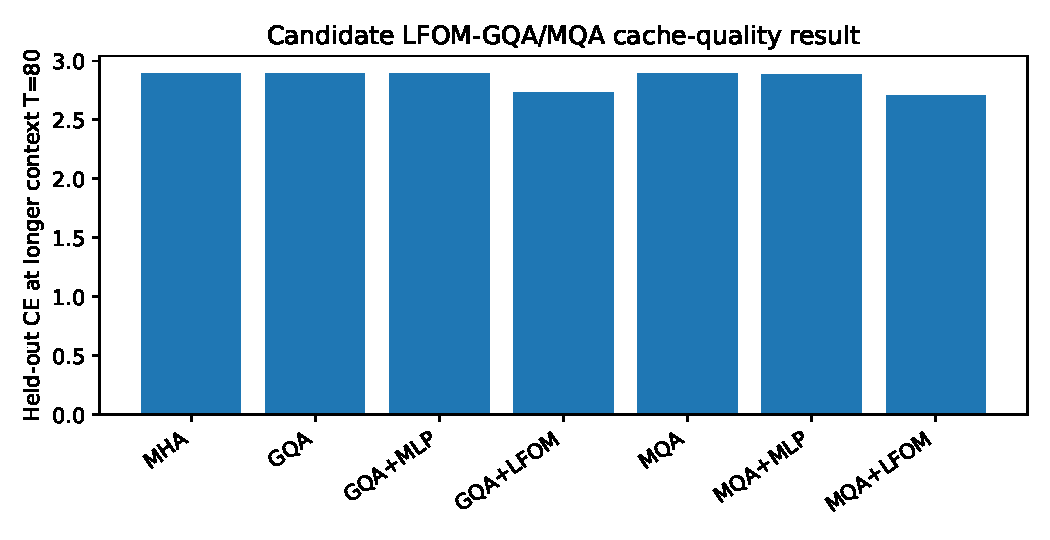
\includegraphics[width=.95\linewidth]{ce80_bar.pdf}
\caption{Held-out CE at longer context $T=80$. LFOM repair improves both GQA and MQA and beats the full-cache MHA baseline in the CPU-scale run.}
\label{fig:ce80}
\end{figure}

\begin{figure}[t]
\centering
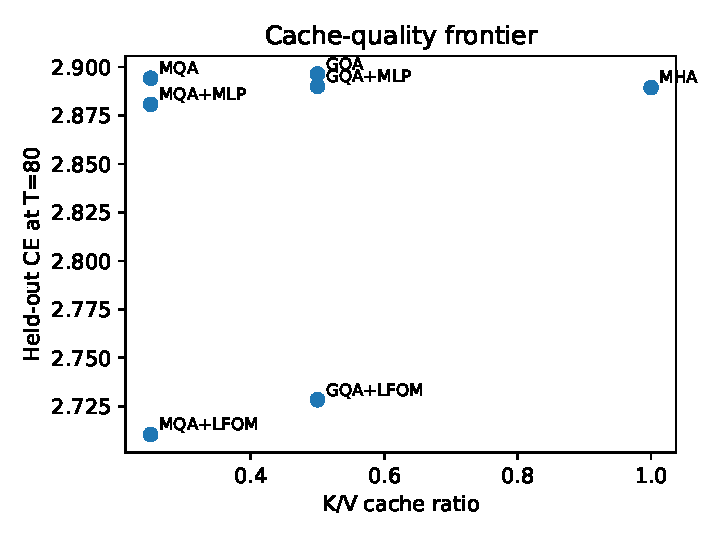
\includegraphics[width=.95\linewidth]{cache_frontier.pdf}
\caption{Cache-quality frontier at $T=80$. The result to scale is the quarter-cache point: MQA+LFOM has lower CE than full-cache MHA in the small LM run.}
\label{fig:frontier}
\end{figure}

\subsection{LoRA and MoE supporting results}
The LoRA experiments remain a practical supporting pillar. In the larger frozen-OPT representation benchmark, LFOM-16 beats AdamW-100 on 186/240 paired episodes, and LFOM+SGD beats AdamW-100 on 219/240 episodes. The strongest interpretation is a warm start: LFOM gives strong early adapter motion, then AdamW, SGD, or Lion can continue.

The MoE experiments remain a systems supporting pillar. In 13,200 streaming route chunks, LFOM route memory reaches oracle-level route MSE in abrupt and drift settings and remains close under scarce-prefix evidence. The route is a small test-time state. LFOM supplies filtering memory for it.


\section{Google Colab GPU validation}\label{sec:colab}
The cache-quality claim must be tested on larger decoder LMs. The repository contains a Colab-ready implementation that trains or uptrains MHA, GQA, MQA, GQA+MLP, MQA+MLP, GQA+LFOM, and MQA+LFOM. It reports validation CE, perplexity, accuracy, long-context CE, K/V cache fraction, throughput, and paired wins. The commands live in \texttt{scripts/run\_gpu\_cache\_frontier.sh}; the paper records the intended experimental grid.

\begin{table}[t]
\centering
\caption{Colab validation grid. The smoke run checks the code path. The small run is intended for a T4 or L4. The full run is intended for Colab Pro or a comparable GPU.}
\scriptsize
\begin{tabular}{lccc}
\toprule
Setting & Smoke & Small & Full \\
\midrule
Seeds & 1 & 1 & 3 \\
Layers & 2 & 4 & 6 \\
Heads & 2 & 4 & 8 \\
Width & 128 & 256 & 512 \\
Context & 64 & 256 & 512 \\
Teacher steps & 10 & 1000 & 4000 \\
Uptrain steps & 5 & 300 & 1000 \\
Dataset & tiny & WikiText & WikiText \\
Output & code check & first signal & main table \\
\bottomrule
\end{tabular}
\label{tab:colab-grid}
\end{table}

The GPU run must use the same seven methods as the CPU run: MHA, GQA, MLP repair, LFOM repair, MQA, MQA+MLP, and MQA+LFOM. The strict win condition is:
\begin{enumerate}[leftmargin=*,itemsep=1pt]
\item LFOM-GQA or LFOM-MQA matches or beats MHA on validation CE and long-context CE.
\item It uses 25--50\% of the K/V cache.
\item It beats the MLP repair control in paired seeds.
\item It gives a better quality-per-cache or quality-per-throughput frontier.
\end{enumerate}
If all four hold, the result becomes the main top-tier claim. If not, the paper should report the small-scale result as a mechanism and leave the cache-compression claim as a direction.

\paragraph{Colab checklist.} The repository root contains a short run file. In Colab, upload the zip, unzip it, install the requirements, run the smoke test, then run the small or full grid. The key output files are \texttt{summary.csv}, \texttt{raw.csv}, \texttt{paired\_wins.csv}, and \texttt{README\_REPORT.md}.

\section{What should be claimed now}
The current evidence supports a clear candidate claim:
\begin{quote}
\emph{K/V-head compression removes useful state. Recurrent first-order memory can restore that state better than nonrecurrent repair in small end-to-end language models.}
\end{quote}
The broader claim, that LFOM-GQA/MQA matches full MHA at 25--50\% K/V cache in large decoder LMs, should only be made after the Colab or GPU run fills the validation table.

\section{Conclusion}
The small-state theory gives one mathematical frame for adapters, routers, and attention memories. The most promising route to a top-tier result is now the attention-compression problem. The concise message is:
\begin{center}
\fbox{\parbox{0.92\linewidth}{Use fewer K/V heads, but give the compressed state first-order memory.}}
\end{center}
The CPU-scale result is strong enough to justify the GPU run. The Colab protocol is included so that the cache-quality claim can be tested without changing the experimental design.

\begin{thebibliography}{99}
\bibitem[Ahn et~al.(2024)]{ahn2024transformers}
Ahn, K., Cheng, X., Daneshmand, H., and Sra, S. (2024). Transformers learn gradient descent in-context.

\bibitem[Ainslie et~al.(2023)]{ainslie2023gqa}
Ainslie, J., Lee-Thorp, J., de~Jong, M., Zemlyanskiy, Y., Lebron, F., and Sanghai, S. (2023). GQA: Training generalized multi-query Transformer models from multi-head checkpoints. \emph{arXiv:2305.13245}.

\bibitem[Dutta and Sra(2024)]{dutta2024lfom}
Dutta, S. and Sra, S. (2024). Learning linear first-order methods with memory-augmented Transformers.

\bibitem[Fedus et~al.(2022)]{fedus2022switch}
Fedus, W., Zoph, B., and Shazeer, N. (2022). Switch Transformers: Scaling to trillion parameter models with simple and efficient sparsity. \emph{JMLR}.

\bibitem[Hu et~al.(2021)]{hu2021lora}
Hu, E.~J., Shen, Y., Wallis, P., Allen-Zhu, Z., Li, Y., Wang, S., Wang, L., and Chen, W. (2021). LoRA: Low-rank adaptation of large language models. \emph{arXiv:2106.09685}.

\bibitem[Moonshot AI(2025)]{kimi2025}
Moonshot AI (2025). Kimi Linear: An expressive, efficient attention architecture. \emph{arXiv:2510.26692}.

\bibitem[Shazeer et~al.(2017)]{shazeer2017moe}
Shazeer, N., Mirhoseini, A., Maziarz, K., Davis, A., Le, Q., Hinton, G., and Dean, J. (2017). Outrageously large neural networks: The sparsely-gated mixture-of-experts layer. \emph{arXiv:1701.06538}.
\end{thebibliography}
\end{document}
